% Options for packages loaded elsewhere
\PassOptionsToPackage{unicode}{hyperref}
\PassOptionsToPackage{hyphens}{url}
%
\documentclass[
]{article}
\usepackage{amsmath,amssymb}
\usepackage{lmodern}
\usepackage{ifxetex,ifluatex}
\ifnum 0\ifxetex 1\fi\ifluatex 1\fi=0 % if pdftex
  \usepackage[T1]{fontenc}
  \usepackage[utf8]{inputenc}
  \usepackage{textcomp} % provide euro and other symbols
\else % if luatex or xetex
  \usepackage{unicode-math}
  \defaultfontfeatures{Scale=MatchLowercase}
  \defaultfontfeatures[\rmfamily]{Ligatures=TeX,Scale=1}
\fi
% Use upquote if available, for straight quotes in verbatim environments
\IfFileExists{upquote.sty}{\usepackage{upquote}}{}
\IfFileExists{microtype.sty}{% use microtype if available
  \usepackage[]{microtype}
  \UseMicrotypeSet[protrusion]{basicmath} % disable protrusion for tt fonts
}{}
\makeatletter
\@ifundefined{KOMAClassName}{% if non-KOMA class
  \IfFileExists{parskip.sty}{%
    \usepackage{parskip}
  }{% else
    \setlength{\parindent}{0pt}
    \setlength{\parskip}{6pt plus 2pt minus 1pt}}
}{% if KOMA class
  \KOMAoptions{parskip=half}}
\makeatother
\usepackage{xcolor}
\IfFileExists{xurl.sty}{\usepackage{xurl}}{} % add URL line breaks if available
\IfFileExists{bookmark.sty}{\usepackage{bookmark}}{\usepackage{hyperref}}
\hypersetup{
  pdftitle={Relatórios em RMarkdown},
  hidelinks,
  pdfcreator={LaTeX via pandoc}}
\urlstyle{same} % disable monospaced font for URLs
\usepackage[margin=1in]{geometry}
\usepackage{color}
\usepackage{fancyvrb}
\newcommand{\VerbBar}{|}
\newcommand{\VERB}{\Verb[commandchars=\\\{\}]}
\DefineVerbatimEnvironment{Highlighting}{Verbatim}{commandchars=\\\{\}}
% Add ',fontsize=\small' for more characters per line
\usepackage{framed}
\definecolor{shadecolor}{RGB}{248,248,248}
\newenvironment{Shaded}{\begin{snugshade}}{\end{snugshade}}
\newcommand{\AlertTok}[1]{\textcolor[rgb]{0.94,0.16,0.16}{#1}}
\newcommand{\AnnotationTok}[1]{\textcolor[rgb]{0.56,0.35,0.01}{\textbf{\textit{#1}}}}
\newcommand{\AttributeTok}[1]{\textcolor[rgb]{0.77,0.63,0.00}{#1}}
\newcommand{\BaseNTok}[1]{\textcolor[rgb]{0.00,0.00,0.81}{#1}}
\newcommand{\BuiltInTok}[1]{#1}
\newcommand{\CharTok}[1]{\textcolor[rgb]{0.31,0.60,0.02}{#1}}
\newcommand{\CommentTok}[1]{\textcolor[rgb]{0.56,0.35,0.01}{\textit{#1}}}
\newcommand{\CommentVarTok}[1]{\textcolor[rgb]{0.56,0.35,0.01}{\textbf{\textit{#1}}}}
\newcommand{\ConstantTok}[1]{\textcolor[rgb]{0.00,0.00,0.00}{#1}}
\newcommand{\ControlFlowTok}[1]{\textcolor[rgb]{0.13,0.29,0.53}{\textbf{#1}}}
\newcommand{\DataTypeTok}[1]{\textcolor[rgb]{0.13,0.29,0.53}{#1}}
\newcommand{\DecValTok}[1]{\textcolor[rgb]{0.00,0.00,0.81}{#1}}
\newcommand{\DocumentationTok}[1]{\textcolor[rgb]{0.56,0.35,0.01}{\textbf{\textit{#1}}}}
\newcommand{\ErrorTok}[1]{\textcolor[rgb]{0.64,0.00,0.00}{\textbf{#1}}}
\newcommand{\ExtensionTok}[1]{#1}
\newcommand{\FloatTok}[1]{\textcolor[rgb]{0.00,0.00,0.81}{#1}}
\newcommand{\FunctionTok}[1]{\textcolor[rgb]{0.00,0.00,0.00}{#1}}
\newcommand{\ImportTok}[1]{#1}
\newcommand{\InformationTok}[1]{\textcolor[rgb]{0.56,0.35,0.01}{\textbf{\textit{#1}}}}
\newcommand{\KeywordTok}[1]{\textcolor[rgb]{0.13,0.29,0.53}{\textbf{#1}}}
\newcommand{\NormalTok}[1]{#1}
\newcommand{\OperatorTok}[1]{\textcolor[rgb]{0.81,0.36,0.00}{\textbf{#1}}}
\newcommand{\OtherTok}[1]{\textcolor[rgb]{0.56,0.35,0.01}{#1}}
\newcommand{\PreprocessorTok}[1]{\textcolor[rgb]{0.56,0.35,0.01}{\textit{#1}}}
\newcommand{\RegionMarkerTok}[1]{#1}
\newcommand{\SpecialCharTok}[1]{\textcolor[rgb]{0.00,0.00,0.00}{#1}}
\newcommand{\SpecialStringTok}[1]{\textcolor[rgb]{0.31,0.60,0.02}{#1}}
\newcommand{\StringTok}[1]{\textcolor[rgb]{0.31,0.60,0.02}{#1}}
\newcommand{\VariableTok}[1]{\textcolor[rgb]{0.00,0.00,0.00}{#1}}
\newcommand{\VerbatimStringTok}[1]{\textcolor[rgb]{0.31,0.60,0.02}{#1}}
\newcommand{\WarningTok}[1]{\textcolor[rgb]{0.56,0.35,0.01}{\textbf{\textit{#1}}}}
\usepackage{longtable,booktabs,array}
\usepackage{calc} % for calculating minipage widths
% Correct order of tables after \paragraph or \subparagraph
\usepackage{etoolbox}
\makeatletter
\patchcmd\longtable{\par}{\if@noskipsec\mbox{}\fi\par}{}{}
\makeatother
% Allow footnotes in longtable head/foot
\IfFileExists{footnotehyper.sty}{\usepackage{footnotehyper}}{\usepackage{footnote}}
\makesavenoteenv{longtable}
\usepackage{graphicx}
\makeatletter
\def\maxwidth{\ifdim\Gin@nat@width>\linewidth\linewidth\else\Gin@nat@width\fi}
\def\maxheight{\ifdim\Gin@nat@height>\textheight\textheight\else\Gin@nat@height\fi}
\makeatother
% Scale images if necessary, so that they will not overflow the page
% margins by default, and it is still possible to overwrite the defaults
% using explicit options in \includegraphics[width, height, ...]{}
\setkeys{Gin}{width=\maxwidth,height=\maxheight,keepaspectratio}
% Set default figure placement to htbp
\makeatletter
\def\fps@figure{htbp}
\makeatother
\setlength{\emergencystretch}{3em} % prevent overfull lines
\providecommand{\tightlist}{%
  \setlength{\itemsep}{0pt}\setlength{\parskip}{0pt}}
\setcounter{secnumdepth}{-\maxdimen} % remove section numbering
\ifluatex
  \usepackage{selnolig}  % disable illegal ligatures
\fi

\title{Relatórios em RMarkdown}
\author{}
\date{\vspace{-2.5em}}

\begin{document}
\maketitle

\hypertarget{referuxeancias-de-rmarkdown}{%
\section{Referências de RMarkdown}\label{referuxeancias-de-rmarkdown}}

\hypertarget{exemplos}{%
\section{Exemplos}\label{exemplos}}

\begin{itemize}
\tightlist
\item
  \textbf{Blogs}

  \begin{itemize}
  \tightlist
  \item
    \href{https://blogs.rstudio.com/ai/}{RStudio AI Blog}
  \item
    \href{https://athospd.github.io/SSC5890/}{Lista de Exercícios}
  \end{itemize}
\item
  \textbf{Livros}

  \begin{itemize}
  \tightlist
  \item
    \href{https://r4ds.had.co.nz/}{R for Data Science}
  \item
    \href{https://livro.curso-r.com/}{Ciência de Dados em R}
  \item
    \href{https://www.tmwr.org/}{Tidy Modeling with R}
  \end{itemize}
\item
  \textbf{dashboard}

  \begin{itemize}
  \tightlist
  \item
    \href{https://curso-r.github.io/202104-intro-ml/exemplos/11-report-credit-data.html}{Exemplinho
    de ML}
  \end{itemize}
\end{itemize}

\hypertarget{o-que-uxe9-o-rmarkdown}{%
\section{O que é o RMarkdown?}\label{o-que-uxe9-o-rmarkdown}}

\begin{Shaded}
\begin{Highlighting}[]
\NormalTok{aloalo }\OtherTok{\textless{}{-}} \DecValTok{2} \SpecialCharTok{+} \DecValTok{2}
\end{Highlighting}
\end{Shaded}

O R Markdown é 4 uma ferramenta para criação de relatórios automatizados
utilizando as linguagem R e Markdown.

A linguagem de marcação Markdown serve para construirmos e formatarmos
diversos formatos de arquivos (PDF, HTML, Word, entre outros) a partir
de um arquivo de texto com regras bem simples. O R Markdown é uma
extensãi di Markdown que nos permite colocar código de R.

Linguagens de marcação utilizam marcadores (símbolos, tags, funções)
para formatar um arquivo de texto simples. Os exemplos mais famosos de
linguagem de marcação são o HTML e LaTeX. I N S Após a construção do
\textbf{documento}, para gerarmos o relatório na extensão desejada,
precisamos \emph{renderizá-lo}, isto é, transformar o arquivo R Markdown
em um PDF, HTML ou Word. Isso pode ser feito no RStudio a partir do
botão \texttt{knit}, que fica logo acima do script, ou pelo atalho
\texttt{CTRL\ +\ SHIFT\ +\ K}.

\hypertarget{regras-simples-de-formatauxe7uxe3o}{%
\subsection{Regras simples de
formatação}\label{regras-simples-de-formatauxe7uxe3o}}

Usando o R Markdown, podemos criar arquivos HTML, PDF e Word sem
precisar sair do R. A grande vantagem é poder de automatização.
Construindo um relatório em R Markdown, com exceção das interpretações e
conclusões, só precisamos montá-lo uma vez. A partir daí, com apenas um
clique podemos:

\begin{itemize}
\item
  replicar o relatório para diversas versões da base de dados
  (modificações, correções, processos periódicos);
\item
  replicar o relatório para diversas variáveis.
\end{itemize}

\hypertarget{marcadores}{%
\subsection{Marcadores}\label{marcadores}}

A seguir, apresentamos uma lista dos principais marcadores utilizados
para formatar texto:

\begin{itemize}
\item
  uma palavra entre asteriscos fica em itálico: \texttt{*texto*} é
  transformado em \emph{texto}
\item
  uma palavra entre dois asteríscos fica em negrito: \texttt{**texto**}
  é transformado em \textbf{texto}
\item
  um ou mais hashtags viram títulos: \texttt{\#\ Título\ muito\ grande},
  \texttt{\#\#\ Título\ grande}, \texttt{\#\#\#\ Título\ médio},
  \texttt{\#\#\#\#\ Título\ pequeno},
  \texttt{\#\#\#\#\#\ Título\ muito\ pequeno}
\item
  hiperlinks podem ser criados com a estrutura
  \texttt{{[}texto{]}(link)}:
\end{itemize}

\texttt{{[}link\ para\ o\ site\ da\ Curso-R{]}(https://curso-r.com)} é
transformado em \href{https://curso-r.com}{link para o site da Curso-R}.

\begin{itemize}
\tightlist
\item
  para deixar o texto com \texttt{esse\ formato} (formato de código),
  apenas coloque o texto entre duas crases.
\end{itemize}

\hypertarget{chunks-escrevendo-nosso-cuxf3digo-de-r}{%
\subsection{Chunks: escrevendo nosso código de
R}\label{chunks-escrevendo-nosso-cuxf3digo-de-r}}

Em um arquivo R Markdown, precisamos escrever nossos códigos dentro dos
\emph{chunks}. Para insirir um chunk, utilize o atalho
\texttt{CTRL\ +\ ALT\ +\ I}.

Dentro dos chunks você poderá escrever códigos em R como se fosse o
nosso script .R tradicional. Por padrão, o código dentro do chunk será
colocado no relatório, assim como o resultado da execução desse código
(i.e., tudo que seria). Veja o exemplo abaixo:

Chunks

\begin{Shaded}
\begin{Highlighting}[]
\NormalTok{meu\_vetor }\OtherTok{\textless{}{-}} \FunctionTok{c}\NormalTok{(}\DecValTok{1}\NormalTok{, }\DecValTok{2}\NormalTok{, }\DecValTok{3}\NormalTok{)}
\NormalTok{meu\_vetor }\SpecialCharTok{+} \DecValTok{1}
\end{Highlighting}
\end{Shaded}

\begin{verbatim}
## [1] 2 3 4
\end{verbatim}

Não é apenas o resultado da última linha que é colocada no relatório.
Todo resultado que seria imprimido na tela (Console) também vai para o
relatório. Repare que objetos criados em um chunk ficam disponíveis para
todos os chunks abaixo dele.

\begin{Shaded}
\begin{Highlighting}[]
\NormalTok{meu\_vetor }\SpecialCharTok{+} \DecValTok{1}
\end{Highlighting}
\end{Shaded}

\begin{verbatim}
## [1] 2 3 4
\end{verbatim}

\begin{Shaded}
\begin{Highlighting}[]
\NormalTok{meu\_vetor }\SpecialCharTok{{-}} \DecValTok{1}
\end{Highlighting}
\end{Shaded}

\begin{verbatim}
## [1] 0 1 2
\end{verbatim}

\begin{Shaded}
\begin{Highlighting}[]
\NormalTok{meu\_vetor }\SpecialCharTok{*} \DecValTok{10}
\end{Highlighting}
\end{Shaded}

\begin{verbatim}
## [1] 10 20 30
\end{verbatim}

Para alterar esses comportamentos padrões, utilizamos os parâmetros do
chunk. Os parêmetros são colocados dentro das chaves, na linha que
define o começo do chunk. Esse \texttt{r} que aparece em todos os chunks
representa que o código dentro dele é um código de R.

Para impedir que o código de um chunk apareça no relatório, basta usar o
parâmetro \texttt{echo\ =\ FALSE}. As chaves neste caso ficaria
\texttt{\{r,\ echo\ =\ FALSE\}}. Quando fazemos isso, apenas o resultado
é mostrado no relatório.

\begin{verbatim}
## [1] 2 3 4
\end{verbatim}

Também podemos impedir que um chunk seja avaliado, mostrando apenas o
código no relatório, usando o argumento \texttt{eval\ =\ FALSE}.

\begin{Shaded}
\begin{Highlighting}[]
\NormalTok{meu\_vetor }\SpecialCharTok{+} \DecValTok{1}
\end{Highlighting}
\end{Shaded}

Por fim, podemos rodar o chunk sem colocar nem o código nem o resultado
no relatório usando o arqumento \texttt{include\ =\ FALSE}. Isso pode
ser utilizado para carregar pacotes, definir funções ou fazer qualquer
tipo de operação auxiliar que o leitor do relatório não precisa saber.

Para saber mais sobre os parâmetros dos chunks, consulte
\href{https://www.rstudio.com/wp-content/uploads/2015/03/rmarkdown-reference.pdf}{este
guia} (inglês).

\hypertarget{importanto-dados}{%
\subsection{Importanto dados}\label{importanto-dados}}

Você pode carregar pacotes e dados normalmente dentro de um script R
Markdown.

\begin{Shaded}
\begin{Highlighting}[]
\FunctionTok{library}\NormalTok{(tidyverse)}
\FunctionTok{library}\NormalTok{(readxl)}
\NormalTok{imdb }\OtherTok{\textless{}{-}} \FunctionTok{read\_csv}\NormalTok{(}\StringTok{"https://raw.githubusercontent.com/curso{-}r/202005{-}r4ds{-}1/master/dados/imdb.csv"}\NormalTok{)}
\end{Highlighting}
\end{Shaded}

Veja que as mensagens e warnings dos nossos códigos também são colocadas
no relatório. Para evitar isso, basta usarmos os parâmetros
\texttt{message=FALSE} e \texttt{warning=FALSE}.

Você precisa carregar o pacote apenas uma vez em cada documento. Uma vez
carregado um pacote, suas funçõe estarão disponíveis para todo código em
R abaixo, no mesmo ou em outros chunks.

\hypertarget{incluindo-tabelas}{%
\subsection{Incluindo tabelas}\label{incluindo-tabelas}}

A função \texttt{knit::kable()} é muito útil para gerar tabelas bem
formatadas.

A seguir, mostramos os 10 filmes com maior lucro na base.

\begin{Shaded}
\begin{Highlighting}[]
\NormalTok{imdb }\SpecialCharTok{\%\textgreater{}\%} 
  \FunctionTok{mutate}\NormalTok{(}\AttributeTok{lucro =}\NormalTok{ receita }\SpecialCharTok{{-}}\NormalTok{ orcamento) }\SpecialCharTok{\%\textgreater{}\%} 
  \FunctionTok{top\_n}\NormalTok{(}\DecValTok{10}\NormalTok{, lucro) }\SpecialCharTok{\%\textgreater{}\%} 
  \FunctionTok{arrange}\NormalTok{(lucro) }\SpecialCharTok{\%\textgreater{}\%}
  \FunctionTok{mutate}\NormalTok{(}
    \AttributeTok{pos =} \DecValTok{10}\SpecialCharTok{:}\DecValTok{1}\NormalTok{,}
    \AttributeTok{lucro =}\NormalTok{ scales}\SpecialCharTok{::}\FunctionTok{dollar}\NormalTok{(lucro)}
\NormalTok{  ) }\SpecialCharTok{\%\textgreater{}\%} 
  \FunctionTok{select}\NormalTok{(}\StringTok{\textasciigrave{}}\AttributeTok{Posição}\StringTok{\textasciigrave{}} \OtherTok{=}\NormalTok{ pos, }\AttributeTok{Filme =}\NormalTok{ titulo, }\AttributeTok{Lucro =}\NormalTok{ lucro) }\SpecialCharTok{\%\textgreater{}\%} 
\NormalTok{  knitr}\SpecialCharTok{::}\FunctionTok{kable}\NormalTok{()}
\end{Highlighting}
\end{Shaded}

\begin{longtable}[]{@{}rll@{}}
\toprule
Posição & Filme & Lucro \\
\midrule
\endhead
10 & The Hunger Games & \$329,999,255 \\
9 & The Dark Knight & \$348,316,061 \\
8 & Star Wars: Episode I - The Phantom Menace & \$359,544,677 \\
7 & The Lion King & \$377,783,777 \\
6 & The Avengers & \$403,279,547 \\
5 & E.T. the Extra-Terrestrial & \$424,449,459 \\
4 & Star Wars: Episode IV - A New Hope & \$449,935,665 \\
3 & Titanic & \$458,672,302 \\
2 & Jurassic World & \$502,177,271 \\
1 & Avatar & \$523,505,847 \\
\bottomrule
\end{longtable}

\hypertarget{incluindo-gruxe1ficos}{%
\subsection{Incluindo gráficos}\label{incluindo-gruxe1ficos}}

Para construir gráficos, não há segredos. O mesmo gráfico que apareceria
na aba \textbf{Plots} do RStudio aparecerá no relatório.

\begin{figure}

{\centering 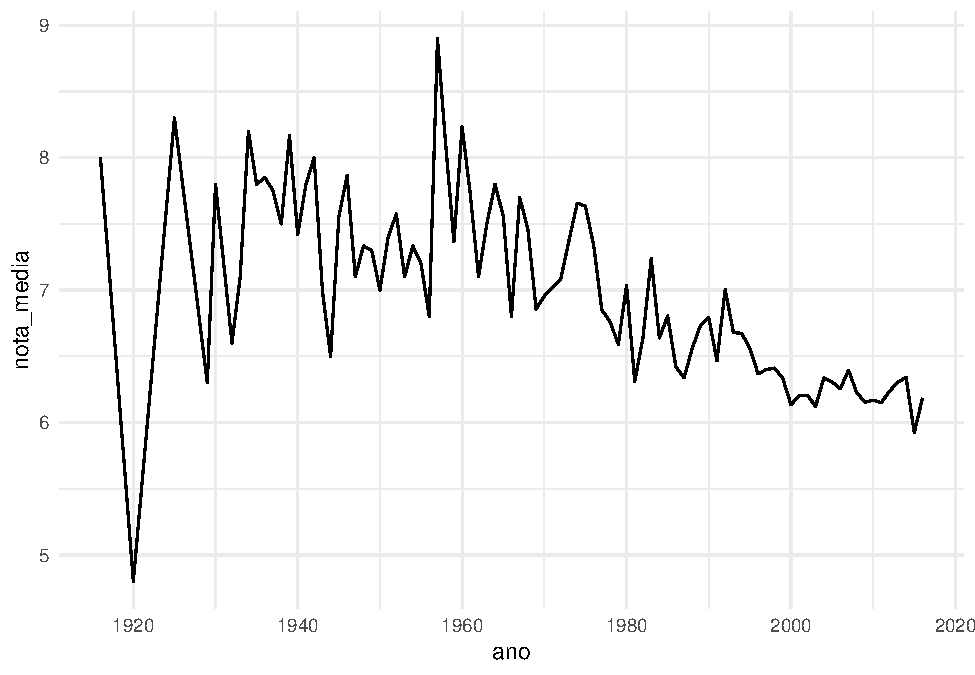
\includegraphics{01-intro-rmarkdown_files/figure-latex/unnamed-chunk-9-1} 

}

\caption{Figura 1. Nota média ao longo dos anos.}\label{fig:unnamed-chunk-9}
\end{figure}

Para centralizar o gráfico no documento, você pode usar o parâmetro
\texttt{fig.align\ =\ "center"} no chunk. Para alterar o tamanho da
figura, existem os parâmetros \texttt{fig.width} (comprimento) e
\texttt{fig.height} (altura). O parâmetro \texttt{fig.cap} coloca
legendas.

\end{document}
